\documentclass[aspectratio=169]{beamer}
\beamertemplatenavigationsymbolsempty

\mode<presentation>
{
	\usetheme{Singapore}
	\setbeamercovered{transparent}
	\setbeamertemplate{footline}[frame number]
}

% \usepackage{flashmovie}
\usepackage[utf8]{inputenc}
\usepackage[T1]{fontenc}
%\usepackage[ngerman]{babel}
\usepackage[english]{babel}
\usepackage{amsmath}
\usepackage[absolute,overlay]{textpos}

\usebackgroundtemplate{%
\begin{tikzpicture}[remember picture,overlay]
\node[anchor=south west] at (current page.south west) {\includegraphics[height=0.4cm]{by.eps}};
\end{tikzpicture}}

\author{Anton Kuzmin}

\institute[]
{
%	Informatik 3 / Rechnerarchitektur\\
%	Universität Erlangen Nürnberg
}
\date{@DATE@}

\usepackage{tikz}

\title{Port luajit to RISC-V}
\subtitle{Motivation, first steps and perspectives}

\setbeamerfont{table font}{size=\tiny}

\begin{document}

\begin{frame}
  \titlepage
\end{frame}

\section{Intro}

\begin{frame}
  \frametitle{Who am I\dots}
  \begin{itemize}
  \item not really a software developer\\
    \dots but write code sometimes
  \item developing embedded systems for 25 years
  \item VME, CompactPCI, AdvancedTCA, SoM
  \item FPGA and SoC-FPGA (Altera/Intel, Microsemi/Microchip)
  \item VHDL (RTL-code, no, it is not a software)
  \end{itemize}
  \vskip.5cm

  My usual problem with the software is how to make it run on a
  hardware which is known not to be working yet and how to bring-up
  and test this hardware. With a soft-core CPU it is getting even
  worse.

\end{frame}


\frame{\tableofcontents[subsectionstyle=show]}

\section{Motivation}

\subsection{Why RISC-V}

\begin{frame}
  \frametitle{Why RISC-V?}

  \begin{minipage}{8.5cm}
  RISC-V (“risk-five”) is an open source Instruction Set Architecture
  (ISA) specification
  \end{minipage}

  \vspace{-1.5cm}
  \begin{flushright}
    
\includegraphics[height=1.5cm]{riscv-logo-1.png}
  \end{flushright}

  \begin{itemize}
    \item open-source, royalty-free
    \item scalable from 32-bit MCU with reduced number of registers
    (rv32e) to multi-core 64-bit OoO CPU (and even 128-bit)
    \item proven on FPGAs and silicon tape-outs
    \item modular design with both standard extensions and resever
    encoding space for custom extensions
    \item already used in a products as a soft-core MCU on FPGAs,
    SoC-FPGA with hard-core RISC-V CPU is coming later this year
  \end{itemize}
\end{frame}

\subsection{Why Lua}
\begin{frame}
  \frametitle{Why Lua?}

  Lua is a powerful, efficient, lightweight, embeddable scripting
  language. It supports procedural programming, object-oriented
  programming, functional programming, data-driven programming, and data
  description.

  \vskip.3cm
  \begin{minipage}{10cm}
  \begin{itemize}
    \item simple
    \item interactive
    \item very compact and portable
    \item simple interface to C and, through it, to an underlying hardware
    \item fast (if it really matters)
  \end{itemize}
  \end{minipage}
  \vskip.3cm
  Contemporary replacement for Forth.  First tried on NIOS II for
  optical link transceiver testing and training in 2012.

  \vspace{-5cm}
  \begin{flushright}
    \includegraphics[height=3.5cm]{de4.jpg}
  \end{flushright}

\end{frame}

\subsection{Why luajit}
\begin{frame}
\frametitle{Why \texttt{luajit}?}
LuaJIT is a Just-In-Time Compiler (JIT) for the Lua programming language.

  \begin{itemize}
  \item \textbf{dynamic assembler}
  \begin{itemize}
    \item for experiments with CPU extensions and hardware accelerators
    \item gcc/binutils/llvm are well beyond my comprehension and are
    not suitable for rapid experiments directly on hardware
    \end{itemize}
    \item used in various interesting projects
    \begin{itemize}
    \item LuaRadio (\texttt{https://luaradio.io/})
    \item Tarantool DB (\texttt{https://www.tarantool.io/en/})
    \item luapower (\texttt{https://luapower.com/})
  \end{itemize}

  \item why \textbf{not}
    \begin{itemize}
    \item the project seems to be not actively developed and maintained since 2017
    \item several [non synchronized] forks
    \item stick to Lua 5.1
    \end{itemize}

  \end{itemize}
\end{frame}

\section{luajit}

\begin{frame}
\frametitle{\texttt{luajit} components}
\begin{itemize}
\item dynasm
\item Lua VM (hand-optimized assembler)\\
      the best [hardest] way to learn RISC-V ISA
\item tracing JIT
\item Garbage Collector
\item extensions: FFI, bit-ops, hard \& soft Floating Point support
\end{itemize}
\end{frame}

\section{Status}

\begin{frame}
\frametitle{Current status}
\begin{itemize}
\item running Lua 5.1 on \texttt{spike} and soft-core RISC-V CPU
\item \texttt{git} repository (fork of \texttt{luajit v2.1})
\item \texttt{Makefile} changes
\item \texttt{rv32i} base instruction encoding
\item registers/immediates/labels -- WIP
\item everything else -- TODO
\end{itemize}
\end{frame}

\section{What's next\dots}

\begin{frame}
\frametitle{What to do}
\begin{itemize}
\item write [all] the code:
\begin{itemize}
\item Lua VM on RISC-V assembler
\item GC
\item soft and hard FP support
\item tracing JIT
\end{itemize}
\item tests
\item benchmarks
\end{itemize}
\end{frame}

\begin{frame}
\frametitle{Perspectives}
Interesting stuff to do, when everything above is running
\begin{itemize}
  \item RISC-V J extension -- what language will be the first to shape it?
  \begin{itemize}
    \item Java
    \item JavaScript
    \item C\#
    \item what else?...
  \end{itemize}
  \item hardware-assisted hot trace detection
  \item hardware-assisted memory management/garbage collection
  \item custom ISA extension (accelerator) -- development and testing
  \item to write yet another Forth on dynasm\\
  (then to write yet another assembler on Forth)
\end{itemize}
\end{frame}

\section{Contact info}
\begin{frame}

  \begin{minipage}{7cm}
    \vskip.5cm
    \huge{Thank you!}
    \vskip1cm
    \small{Anton Kuzmin}\\
    \small{\texttt{anton.kuzmin@cs.fau.de}}\\
    \small{\texttt{https://github.com/ak-fau/}}
    \vskip.5cm
    \Huge{Questions?..}
  \end{minipage}

  \vspace{-5cm}
  \begin{flushright}
    \includegraphics[height=5cm]{github-vcard.png}\\
  \end{flushright}

\end{frame}


\end{document}
